\chapter{جمع بندی}
در این قسمت چند نکته‌ی مهم طبق تجربه را بیان می‌کنیم که تعدادی از این نکات در بخش نگارشی و تعدادی دیگر را در بخش تکنیکی را مطرح می‌کنیم. 

\section{نکات نگارشی}
\begin{enumerate}
	\item \textbf{قالب
		\lr{Word} 
		پایان‌نامه:} به منظور آشنایی با نحوه‌ی نگارش پایان‌نامه و قوانین کلی حتما نگاهی به جدید‌ترین نسخه‌ی این قالب و توضیحات آن داشته باشید. 
	\item \textbf{درج یک کلمه به صورت کامل در یک سطر:}
	برخی اوقات می خواهیم یک عبارت به صورت کامل در یک سطر قرار گیردِ، نه اینکه بخشی از آن در انتهای یک سطر و بخش دیگر در ابتدای سطر بعدی. در این مواقع می‌توانیم بین لغات آن عبارت بین درج هیچگونه فاصله‌ای از علامت مد استفاده کنیم. برای مثال  فعل 
	\textit{خواهیم پراخت}
	ممکن است در شرایطی قرار بگیرید که 
	\textit{خواهیم} 
	 در انتهای یک سطر و 
	 \textit{پرداخت}
	 در ابتدای سطر دیگر قرار گیرد. در این صورت با قرار دادن علامت 
	 \verb|~| 
	 میان 
	 \textit{خواهیم} 
	 و 
	 \textit{پرداخت}
	 و بدون هیچگونه فاصله‌ای مشکل حل می‌شود. در حالتیکه یک بخش ریاضی یا هایپرلینک دچار این مشکل شود، از دستور 
	 \verb*|\linebreak| 
	 در یک خط قبل از آن استفاده کنید. در این صورت فاصله‌ها طوری تنظیم می‌شوند که آن بخش به طور کامل در یک خط یکسان قرار گیرد. 
	
	\item \textbf{درج نیم‌فاصله:}
	برای درج نیم‌فاصله اگر از ویندوز استفاده می‌کنید، به راحتی می‌توانید از ترکیب کلید‌های‌ 
	\lr{Shift+Space} 
	استفاده کنید. در نظر داشته باشید برای این باید کیبورد استاندارد فارسی یا 
	\lr{Standard Persian Keyboard} 
	را از قبل نصب کرده باشید. اگر آن را از قبل نصب نکرده‌اید، باید یکسری مراحل را طی کنید. ابتدا وارد 
	\lr{Settings} 
	ویندوز شوید، 
	\lr{Time \& Language} 
	را انتخاب کنید، سپس وارد بخش 
	\lr{Language} 
	شوید.  کلید 
	\lr{Options}
	را بر روی زبان 
	\lr{Persian}
	را انتخاب کنید. در قسمت 
	\lr{Keyboards} 
	گزینه‌ی 
	\lr{Add a Keyboard} 
	و در نهایت زبان 
	\lr{Persian (Standard)} 
	را انتخاب کنید. 
\end{enumerate}	

\section{تکات تکنیکی}
	
\begin{enumerate}
	
	\item \textbf{زیاد بودن تعداد زیر--تصویر‌ها و قرار نگرفتن آن ‌هادر یک صفحه:}
	بعضی مواقع ممکن است چند تصویر داشته باشیم و بخواهم آن‌ها را در کنار هم به صورت 
	\lr{subfigure} 
	قرار دهیم. اگر تعداد تصاویر زیاد باشد، ممکن است همه در یک صفحه جا نشوند و صفحه بهم بریزد. چرا که فرض \lr{\LaTeX}این است که تصویر یا تصاویر قرار داده شده در محیط 
	\lr{figure} 
	باید در یک صفحه جا بشوند. در صورت روبه‌رو شدن با چنین مشکلی می‌توانید چند محیط تصویر بسازید و در ابتدای هر کدام از محیط‌های تصویر غیر از اولین مورد، به صورت زیر عمل کنید. 

	\begin{latin} 
		\verb|\begin{figure}|\\
		\verb|\ContinuedFloat|\\
		\verb|\centering|\\
		other commands \\
		\verb|\end{figure}|\\
	\end{latin} 

\item \textbf{بد ظاهر شدن زیرنویس  تصویر یا بالانویس  جدول در فهرست مربوطه:}
اگر زیرنویس یک  تصویر یا بالانویس یک جدول طولانی باشد یا اگر در آن یک مرجع یا معادلات ریاضی قرار دهید، این متن طولانی، مرجع یا معادله‌ی ریاضی وارد فهرست تصاویر یا جداول شده و جلوه‌ی جالبی نخواهد داشت. به این منظور از دستور زیر برای ایجاد زیرنویس یا بالانویس استفاده کنید. 
\begin{latin}
	\noindent
	\verb*|\caption[short text]{text}|
\end{latin} 
به این صورت که در بخش 
\lr{short text}
یک زیرنویس یا بالانویس کوتاه و مختصر بدون مرجع و یا معادلات ریاضی قرار می‌دهید. زیرنویس یا بالانویس تکمیلی را نیز در بخش 
\lr{text}
می‌نویسید. توجه داشته باشید که متن 
\lr{short text}
متنی خواهد بود که در فهرست تصاویر یا جداول درج می‌شود و متن 
\lr{text} 
در متن اصلی پایان‌نامه در زیرتصویر یا بالای جدول عینا ظاهر می‌شود. همچنین توجه داشته باشید که نباید یک کلمه را در زیرنویس یا بالانویس به صورت پانویس یا علائم اخصاری استفاده کنید. به عبارتی 
از دستور 
\verb|\gls{label}|
و متشقات آن در زیرنویس یا بالانویس استفاده نکنید. در غیر این صورت این پانویس یا کلمه‌ی اختصاری اولین بار خود را در فهرست تصاویر یا جدول نشان خواهد داد که نه تنها زیبایی بلکه کارایی خود را نیز از دست خواهد داد. بدین منظور اگر یک کلمه‌ی اختصاری لاتین دارید یا می‌خواهید از پانویس استفاده کنید، تنها از دستور 
\begin{latin}
	\noindent
	\verb|\lr{<label>}|
\end{latin}
یا دستورات 
\begin{latin}
	\noindent
	\verb|\gls*{<label>}| \\
	\verb|\glspl*{<label>}| \\
\end{latin}
استفاده کنید. 

\item{\textbf{هم طراز نبودن خطوط یک پاراگراف}:
برخی اوقات ممکن است که با مشکل هم طراز نبودن ابتدا و انتهای خطوط یک پاراگراف مواجه شویم. برای حل این مشکل از بسته‌ی 
\lr{ragged2e}
 و دستور 
\verb*|\justifying|
استفاده کنید. برای اطلاعات بیشتر به 
\href{https://www.overleaf.com/learn/latex/Text_alignment}{هم‌طرازی متن در \lr{\LaTeX}}
مراجعه بفرمایید. 
}

\item{\textbf{خطوط سفید خالی ناخواسته در اطراف محیط معادله و مشتفات آن}:
گاهی اوقات هنگام استفاده از محیط‌هایی مانند 
\verb*|align|
و مشابه آن به دلیل زیاد بودن تعداد خطوط معادله و جانشدن آن در صفحه‌ی فعلی، تمامی خطوط آن محیط به صفحه‌ی بعدی منتقل می‌شود و یک ناحیه‌ی سفید خالی ناخواسته در صفحه‌ی قبلی به وجود می‌آید. علت این امر این است که در یک محیط شناور، همانند مشکلی که در مورد اول ۱ اتفاق می‌افتد، امکان شکسته شدن وجود ندارد. یعنی قرار گرفتن بخشی از خطوط معادله در یک صفحه و بخشی دیگر در صفحه‌ی بعدی وجود ندارد و باید تمامی خطوط معادله در یک صفحه قرار گیرند. برای حل این مشکل و امکان جدا شدن خطوط از دستور
\verb*|\allowdisplaybreaks|
در 
\lr{preamble} 
استفاده کنید. توجه داشته باشید که این دستور به کل فایل اعمال می‌شود. اگر هدف اعمال این دستور به صورت ناحیه‌ای دلخواه از متن باشد، از دستورات زیر استفاده بفرمایید.  

\begin{latin}
	\begin{flushleft}
		\begin{verbatim}
			\begingroup
			\allowdisplaybreaks
			\begin{align}
				...
			<equation lines>
				... 
			\end{align}
			\endgroup
		\end{verbatim}
	\end{flushleft}
\end{latin}  
} 

\item {\textbf{سوالات بی پایان در \lr{\LaTeX}: }}
در هنگام استفاده از \lr{\LaTeX} و این برنامه ممکن است، هر شخص به بسته به نوع نوشتار، خواسته و سلیقه به مشکلات و سوالاتی برخورد کند. حتما در ضمن سرچ کردن مشکل خود، وبسایت های زیر را بررسی کنید. 
	\begin{latin}
	\noindent
	\href{https://stackoverflow.com/}{Stackoverflow}\\
	\href{http://parsilatex.com/site/}{ParsiLatex}
\end{latin}
\end{enumerate}	

\section{همانندجویی و ثبت پایان‌نامه/رساله}

در این قسمت به چند نکته در رابطه با نگارش پایان‌نامه/رساله با استفاده از \lr{\LaTeX} و ثبت آن در ایرانداک و همچنین سامانه‌ی پارسه اشاره می‌کنیم. ‍‍

{\colorit{purple}{
توجه داشته باشید که این موارد در 
سال ۱۴۰۰
نوشته شده است و ممکن است در 
سال‌های آتی دستخوش تغییراتی شود، 
پس حتما از تغییرات اعمالی در روند، مقررات و بروز رسانی‌های موجود 
اطلاع کسب بفرمایید.
}}

\begin{enumerate}
\item \textbf{همانندجویی متن نوشته شده به \lr{\LaTeX}در سامانه‌ی ایرانداک:}
یکی از مشکلاتی که ممکن است برای همانندجویی پایان‌نامه نوشته شده به \lr{\LaTeX} پیش آید، چگونگی انجام همانندجویی در سایت 
\href{https://irandoc.ac.ir/}{ایرانداک}
است. برای این منظور حتما فایل ویدویی آپلود شده توسط این سامانه 
به آدرس 
\begin{latin}
	\noindent
	\url{https://tik.irandoc.ac.ir/Home/MembershipGuide}
\end{latin} 
یا مستقیما 
\href{https://www.aparat.com/v/h0ijS}
{فایل ویدیویی آماده‌‌سازی فایل‌ها با فرمت زی پرشین}
را مشاهده کرده و مراحل ذکر شده را طی کنید. 

\item \textbf{ثبت در سامانه‌ی ایرانداک:}
	بنابر پاسخ ایرانداک به سوالات پرکاربرد در بخش سامانه‌ی ملی ثبت و زیربخش ثبت اطلاعات برای 
\href{https://helpdesk.irandoc.ac.ir/Dana/Kb/68-%D9%BE%D8%A7%DB%8C%D8%A7%D9%86%E2%80%8C%D9%86%D8%A7%D9%85%D9%87-%D9%85%D9%86-%D8%A8%D8%A7-%D9%86%D8%B1%D9%85%E2%80%8C%D8%A7%D9%81%D8%B2%D8%A7%D8%B1-%D9%84%D8%A7%D8%AA%DA%A9%D8%B3-%D9%86%D9%88%D8%B4%D8%AA%D9%87-%D8%B4%D8%AF%D9%87-%D8%A7%D8%B3%D8%AA%D8%8C-%DA%86%D9%87-%DA%A9%D9%86%D9%85%D8%9F}{ثبت پایان‌نامه/رساله با فرمت‌ها \lr{\LaTeX}}،
 باید علاوه بر فایل‌
\lr{pdf}
و مجموعه فایل‌های \lr{\LaTeX}، یک فایل ورد به فرمت 
\lr{.docx} 
نیز از 
\textbf{از ابتدای پایان‌نامه/رساله تا پایان فهرست مطالب به همراه فهرست منابع}
را تهیه و بارگذاری فرمایید. تصویر
~\ref{submission-thesis} 
را ببینید. 
\begin{figure}[H]
	\centering
	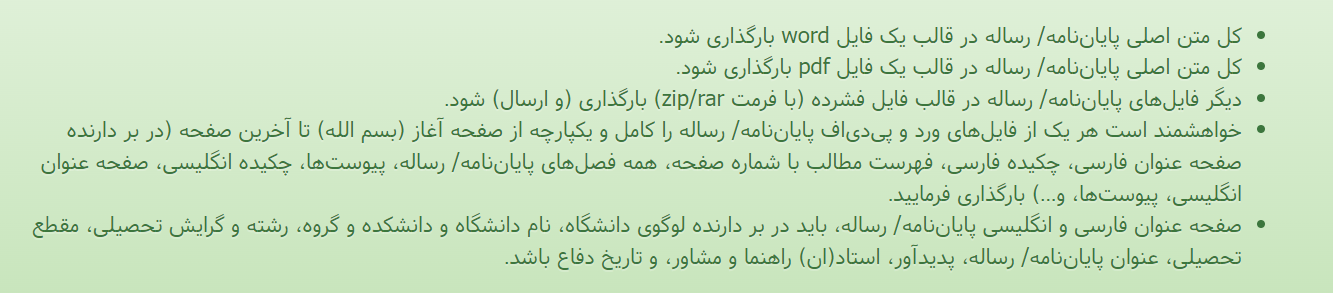
\includegraphics[width = 1\linewidth]{thesis-submission-regulations.png}
	\caption{مقررات مربوط به ثبت پایان‌نامه در ایرانداک} 
	\label{submission-thesis}
\end{figure}


\item \textbf{ثبت در سامانه‌ی 
\href{https://parseh.modares.ac.ir}{پارسه}
:} 
بنابر راهنمای ارسال و بارگذاری پایان‌نامه/رساله در سامانه‌ی پارسه جهت بارگذاری فایل‌های تهیه شده با 
\lr{\LaTeX}،
علاوه بر فایل کامل پایان‌نامه/رساله  با فرمت 
\lr{.pfd}،
یک فایل زیپ شده مربوط به 
\lr{\LaTeX}،
باید یک فایل 
\lr{word} 
 چهار صفحه‌ای به فرمت 
\lr{.doc} 
یا 
\lr{.doxc}
شامل صفحه عنوان فارسی، چکیده‌ی فارسی با کلید واژه‌ها، چکیده‌ی انگلیسی با کلید واژها، صفحه عنوان انگلیسی نیز تهیه و بارگذاری شود. برای اطلاعات بیشتر به 
\linebreak
\href{https://parseh.modares.ac.ir/files/site1/files/guide2.pdf}{راهنمای بارگذاری پایان نامه/ رساله}
مراجعه کنید. 


\item \textbf{مقررات ساختاری در ثبت پایان‌نامه}:
توجه داشته باشید که برای تایید ثبت پایان‌نامه در ایرانداک و همچنین سامانه‌ی پارسه باید حتما پس از صفحه‌ی عنوان، سه فرم را در فایل موجود درج بفرمایید. 
\begin{itemize}
	\item \textbf{برگه‌ی تاییدیه‌ی داوران از جلسه‌ی دفاع:}
توجه داشته باشید این برگه باید توسط استاد راهنما، استاد/اساتید مشاور (در صورت وجود)، نماینده‌ی شورای تحصیلات تکمیلی، داوران داخلی و خارجی به امضا رسیده باشد. 

\item \textbf{آیین‌نامه‌ی حق مالیکت مادی و معنوی:}
		این فرم نیز باید توسط دانشجو تکمیل و امضا شده باشد. 

\item \textbf{آیین‌نامه‌ی حق چاپ :}
		این فرم نیز باید توسط دانشجو تکمیل و امضا شده باشد. 
\end{itemize}
\end{enumerate}	

\noindent
برای دریافت فرم‌های مربوطه به آیین‌نامه‌های ذکر شده در دو مورد آخر به 
\href{https://www.modares.ac.ir/ece/forms}{آدرس فرم‌ها} 
و بخش فرم‌های پژوهشی در دانشکده‌ی مهندسی برق و کامپیوتر دانشگاه تربیت مدرس مراجعه بفرمایید. 
